\documentclass[border=3pt]{standalone}
\usepackage{tikz}
\usetikzlibrary{arrows.meta,calc,positioning}
\tikzset{pin/.style={-{Stealth[length=5pt]}},
  blk/.style={draw, thick, font=\sffamily\small, align=center}}
\begin{document}
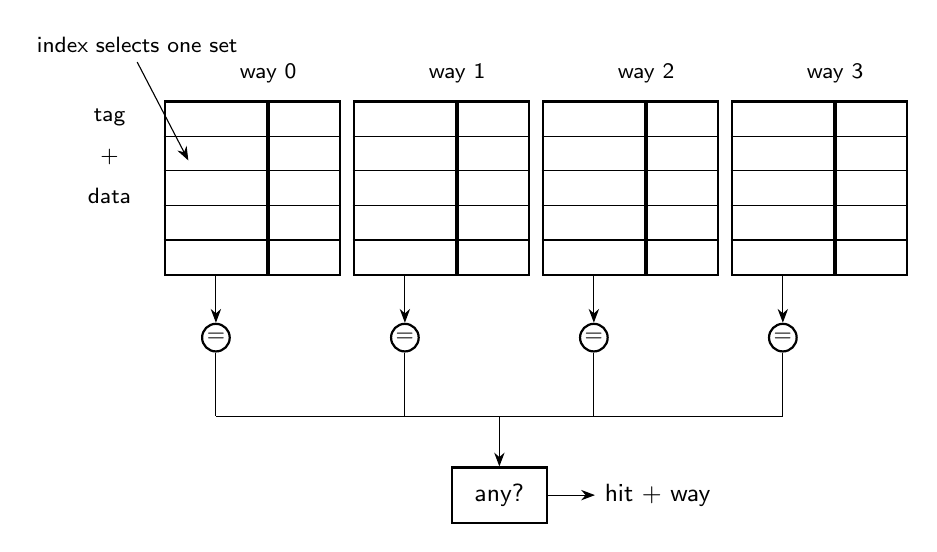
\begin{tikzpicture}[font=\sffamily\small]
  % four ways
  \foreach \i in {0,1,2,3}{
    \node[blk, minimum width=13mm, minimum height=22mm] (t\i) at (2.4*\i,0) {};
    \node[blk, minimum width=9mm, minimum height=22mm, anchor=west] (d\i) at (t\i.east) {};
    \node[font=\sffamily\footnotesize, above=1mm of t\i.north east] {way \i};
    \foreach \y in {-6.6,-2.2,2.2,6.6}{
      \draw ($(t\i.west)+(0,\y mm)$) -- ($(d\i.east)+(0,\y mm)$);}
    \node[draw, thick, circle, inner sep=1pt, font=\footnotesize] (c\i) at (2.4*\i,-1.9) {$=$};
    \draw[pin] (t\i.south) -- (c\i.north);
  }
  \node[font=\sffamily\footnotesize] at (-1.35,0.9) {tag};
  \node[font=\sffamily\footnotesize] at (-1.35,0.4) {+};
  \node[font=\sffamily\footnotesize] at (-1.35,-0.1) {data};
  % set select highlight
  \draw[pin] (-1.0,1.6) node[above, font=\sffamily\footnotesize]{index selects one set} -- (-0.35,0.35);
  % hit OR: comparators drop to a bus, bus feeds the block
  \node[blk, minimum width=12mm, minimum height=7mm] (or) at (3.6,-3.9) {any?};
  \draw (0,-2.9) -- (7.2,-2.9);
  \foreach \i in {0,1,2,3}{\draw (c\i.south) -- (2.4*\i,-2.9);}
  \draw[pin] (3.6,-2.9) -- (or.north);
  \draw[pin] (or.east) -- ++(6mm,0) node[right]{hit + way};
\end{tikzpicture}
\end{document}
